\newpage
\section{Diagramas de Secuencia}
El diagrama de secuencia es el encargado de mostrar la interacción que tiene un conjunto de objetos pertenecientes a una apliación en un cierto lapso de tiempo, en el cual se indican los módulos o clases que forman parte del sistema y las llamadas entre ellos para realizar una tarea específica. Estos diagramas permiten observar la perspectiva cronológica de las interacciónes que tiene el sistema \cite{secuencia}

\subsection{Diagrama de secuencia del sistema}
La Figura \ref{fig:diagramaSecuencia} muestra el diagrama de secuencia del sistema.

\hypertarget{fig:diagramaSecuencia}{
	\begin{figure}[htbp]
		\begin{center}
			\hypertarget{fig:diagramaSecuencia}{
				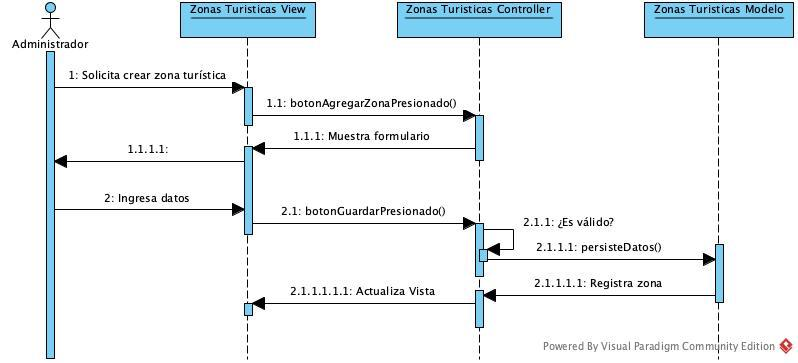
\includegraphics[ scale=.4]{analisisRequerimientos/secuencia/images/diagramaSecuencia}
				\caption{Diagrama de secuencia del sistema}
			}
			\label{fig:diagramaSecuencia}
		\end{center}
	\end{figure}
}